\documentclass[conference]{IEEEtran}
\IEEEoverridecommandlockouts
% The preceding line is only needed to identify funding in the first footnote. If that is unneeded, please comment it out.
\usepackage{cite}
\usepackage{amsmath,amssymb,amsfonts}
\usepackage{algorithmic}
\usepackage{graphicx}
\usepackage{textcomp}
\usepackage{xcolor}
\usepackage{todo}
\usepackage{tikz}
\def\BibTeX{{\rm B\kern-.05em{\sc i\kern-.025em b}\kern-.08em
    T\kern-.1667em\lower.7ex\hbox{E}\kern-.125emX}}

\tikzstyle{block} = [rectangle, draw, 
    text width=5em, text centered, rounded corners, minimum height=2em]
\tikzstyle{oval} = [ellipse, draw, 
    text width=5em, text centered, rounded corners, minimum height=2em]
\tikzstyle{bt} = [rectangle, draw, 
    text width=1em, text centered, rounded corners, minimum height=2em]
\usetikzlibrary{calc}
\usetikzlibrary{arrows.meta}
\usetikzlibrary{positioning}
\usetikzlibrary{fit}
\usetikzlibrary{shapes.geometric}

\begin{document}

\title{VizAPI: Visualizing Interactions between Java Libraries and Clients
\thanks{This work was partially supported by Canada's Natural Science and Engineering Research Council.}
}

\author{\IEEEauthorblockN{1\textsuperscript{st} Sruthi Venkatanarayanan}
\IEEEauthorblockA{\textit{University of Waterloo} \\
Waterloo, ON, CANADA \\
s42venkat@uwaterloo.ca}
\and
\IEEEauthorblockN{2\textsuperscript{nd} Jens Dietrich
\IEEEauthorblockA{\textit{Victoria University of Wellington}\\
Wellington, NZ \\
jens.dietrich@vuw.ac.nz}
\and
\IEEEauthorblockN{3\textsuperscript{rd} Craig Anslow}
\IEEEauthorblockA{\textit{Victoria University of Wellington} \\
Wellington, NZ\\
craig.anslow@ecs.vuw.ac.nz}
\and
\IEEEauthorblockN{4\textsuperscript{th} Patrick Lam}
\IEEEauthorblockA{\textit{University of Waterloo}\\
Waterloo, ON, CANADA\\
patrick.lam@uwaterloo.ca}
}
}

\maketitle

\begin{abstract}
Software projects make use of libraries extensively. Libraries make available intended API surfaces—sets of exposed library interfaces that library developers expect clients to use. However, in practice, clients only use small fractions of intended API surfaces of libraries. We have implemented the VizAPI tool, which shows a visualization that includes both static and dynamic interactions between clients, the libraries they use, and  those libraries’ transitive dependencies (all written in Java). We then present some usage scenarios of VizAPI. One application, by client developers, is to answer a query about upstream code: will their code be affected by breaking changes in library APIs? Additionally, library developers can use VizAPI to find out about downstream code: which APIs in their source code are commonly used by clients? 
\end{abstract}

\begin{IEEEkeywords}
static program analysis,
dynamic program analysis,
API usage,
software evolution,
software maintenance
\end{IEEEkeywords}

\section{Introduction}
\label{sec:introduction}

Virtually all modern software projects use libraries, driven in part by the ease of use of open source component repositories such as Maven and npm. Library developers design Application Programming Interfaces, or APIs, for their libraries, and clients invoke these APIs. APIs typically provide clients with methods that can be invoked, fields that can be accessed, classes that can be instantiated, and annotations that can be used. We use the term ``API surface'' to denote the APIs that a library makes available to other code artifacts (clients and other libraries). It is important that API surfaces are easy to use and are maintainable~\cite{myers-cacm-2016}.

The number of dependencies used by modern software has exploded, and so has their complexity~\cite{kikas2017structure,benelallam2019maven}: deeper, transitive dependencies are now common, components are upgraded more frequently, and developers increasingly struggle to deal with issues arising from those changes. Issues include: (1) dealing with conflicting versions of the same component (also known as dependency hell) and dealing with supply chain vulnerabilities of deep dependencies (often notified by bots creating pull requests); (2) new issues around security and resilience of the software supply chains, e.g. problems with changes to commodity components (as in the infamous left-pad incident~\cite{collins16:_how}) and novel attack patterns like typosquatting; and, (3) the use of unnecessary, bloated, and trivial dependencies~\cite{abdalkareem2017developers,soto2021comprehensive}.

The benefits of using libraries (e.g. the ease of including functionality that one is not responsible for maintaining) are thus offset by the issues mentioned above. 
Let's consider one other issue: breaking changes. \textit{Potentially} breaking changes in library APIs are common~\cite{dietrich2014broken,raemaekers2014semantic}. However, any library change is only potentially breaking; does it \textit{actually} break any particular client? Only if a client uses a specific component API with an incompatible change.

We now discuss a possible usage scenario, that could be beneficial to client developers. First, consider a client \textit{C}, and a library \textit{L}. Consider that \textit{L} has packages \textit{L}\textsubscript{1}, \textit{L}\textsubscript{2} and 
\textit{L}\textsubscript{3}. \textit{C} calls into \textit{L}\textsubscript{1} and \textit{L}\textsubscript{2}. Internally in \textit{L}, \textit{L}\textsubscript{1} and \textit{L}\textsubscript{2} call into each other, but not into \textit{L}\textsubscript{3}. From our visualization 
of this system, it is easy to tell that any breaking changes in \textit{L}\textsubscript{3} should not affect \textit{C}. Also consider that \textit{L}\textsubscript{3} uses an external dependency \textit{D}. We can say that \textit{C} does not require \textit{D} to be on its classpath.

In many programming environments, including Java/Maven, a client developer's decision to use a particular API is a local decision, taken by the developer as they build their system. To our knowledge, there are no existing systems that help developers visualize which APIs are used throughout an entire project. We claim that such a visualization has potential applications for both client and library developers.

From the library developer side, under plain Java (i.e. no runtime containers) and considering reflection, the effective API surface of any component is huge. Essentially: every method can be called, and every field can be read and written. Even considering only the published API surface (methods, fields, classes, and annotations with the correct visibility modifiers), libraries' API surfaces still often have hundreds to thousands of members. The breadth of the API surface is a liability with respect to continued maintenance of the library; many developers aspire to avoid breaking changes by preserving, whenever possible, library behaviour that is depended on by clients. Knowing that few clients use a particular API would be valuable.

On the other hand, we would expect (and have verified in other work) that each client uses only a small portion of each of its dependencies' API surfaces. Consider breaking changes again. GitHub provides the Dependabot tool~\cite{mullans20:_keep_depen}, which monitors for upstream changes and automatically proposes pull requests to update dependency versions. That tool may well pull in breaking changes. However, we hypothesize that, most of the time, most breaking changes will not affect most clients; it is useful for clients to know whether they are using the parts of the API surface that are subject to a particular breaking change. A client with broad dependencies on a library (uses a larger fraction of its API surface) is more likely to be affected by its changes than a client with narrow dependencies (smaller fraction). A narrow library dependency would also suggest that it would be easier to swap the library for a functionally similar replacement.

Additionally, as researchers, we would like to understand how library
APIs are used by clients more generally. Zhong and
Mei~\cite{zhong19:_empir_study_api_usages} investigated API usages in
a dataset of 7 experimental subjects (clients) and the libraries that
they depend on.  They found that clients use less than 10\% of the
declared APIs in libraries. Our visualization allows developers and
researchers to visualize distribution information about how different
parts of clients use different parts of libraries.

This paper presents the VizAPI tool, which shows visualization overviews showing API usages---from clients to libraries, but also between libraries (including transitive dependencies). VizAPI incorporates information from static and dynamic analyses. We intend to make VizAPI publicly available.

[Let's put as short an example as we can here, including a picture].

Our contributions include:
\begin{itemize}
\item an implementation of the VizAPI tool, which presents a visualization of API usage information; VizAPI collects static information and instruments Java code and collect dynamic instrumentation information about API uses in practice and presents it as a d3 visualization (Section~\ref{sec:collecting-data}--\ref{sec:vis-system});
\item a discussion of VizAPI usage scenarios (Section~\ref{sec:evaluation}) based on a collection of 11 libraries and 38 clients.
\end{itemize}

%VizAPI usage scenarios, which we discuss in Section~\ref{sec:discussion}, include guidance to API designers, based on the fact that API usages are sparse, as well as suggestions for tool designers.

%To expand on our aims, we aim to characterize (1) API uses of libraries that are not anticipated by the library developers (``mis-uses'') as well as (2) the empirical extent of API uses by their clients (``API surfaces''). 

%% {\bf Findings.} Our results indicate that API mis-uses are generally rare: developers respect modularity declarations and seldom use reflection to bypass access modifiers (with serialization as a key exception). On the other hand, clients use widely varying portions of their libraries.



%% As a second problem, consider the detection of vulnerabilities in dependencies. Detection is relatively straight-forward: compute the transitive closure of all dependencies, and cross-reference the transitive dependencies with vulnerability databases like CVEs. Tools like \textit{snyk} and \textit{dependabot} are based on this general idea. Some languages and build systems like npm have built-in language-specific support (\textit{npm audit}). The problem is again precision---listing something as a dependency does not mean that all of its functionality is used. So, if dependencies are sufficiently large and deep, a conservative approach inevitably results in false positives. Indeed, Elizalde Zapata et al~\cite{elizalde18:_towar_smoot_librar_migrat} found that 73\% of their studied clients with theoretically vulnerable dependencies were not actually at risk from CVEs in those dependencies, and Chinthanet et al~\cite{chinthanet20:_code_based_vulner_detec_node} implemented a code-based vulnerability detection tool for Node.js applications. Like the boy who cried wolf, false positives can lead to a potentially devastating impact on application security when true positives start being ignored, as demonstrated in the infamous Equifax incident~\cite{luszcz2018apache}. Sadowski et al~\cite{sadowski2018lessons}, among others, also cite the necessity for low false positive rates in developer tools.

%% The basic problem is well-known. In the history of Java (and other languages), several constructs enable component developers to better define and enforce the API surface, including access modifiers, modules, and bundles restricting access to packages, and packaging of components that only expose ``services'', i.e. instantiable classes implementing some abstract type that specifies the service. However, these restrictions always have to compete with the need to provide runtime introspection and code generation features.  Such features are needed to write generic software that can adapt to its usage context. A good example is the automated mapping of domain models to persistency (XML, JSON, RDMBMS, etc).

%  This is often part of another successful trend in modern software engineering---convention over configuration---where services are inferred based on implicit interfaces defined by conventions. 

%In a sense, this has created an arms race:  technologies trying to control APIs versus techniques allowing software to bypass restrictions. This is the space that developers have to navigate when writing modern software.


\section{Related Work}
\label{sec:related-work}
A representative tool from the software visualization literature is
CodeSurveyor, by Hawes et al~\cite{hawes15:_codes}. This tool visualizes large
codebases using cartographic maps as an analogy.  While it
incorporates dependency information into the layout of the map, VizAPI
differs from CodeSurveyor as it focusses on usage relationships
between different modules---primarily API invocations---using test
cases to identify relationships between clients and libraries, rather
than investigating an entire system, as CodeSurveyor does.  Earlier
work in the same vein is the software cartography project by Kuhn et
al~\cite{kuhn10:_softw} and by DeLine~\cite{deline05:_stayin}.

% could mention
%software visualization/history animation:

%Gource
%code_swarm https://effectivesoftwaredesign.com/2012/05/24/code-swarm-visualizing-the-evolution-of-software-systems/


There is a large body of work investigating API usages, particularly
in mining API specifications, as first introduced by Ammons et
al~\cite{AmmonsETAL02MiningSpecifications}. Closer to the present work
is that by Zhong and Mei~\cite{zhong19:_empir_study_api_usages}, who
have investigated API usages in a dataset of 7 experimental subjects
(clients) and the libraries that they depend on. Some of those
findings are relevant to us: they find that clients use less than 10\%
of the declared APIs in libraries. Saied et
al~\cite{saied15:_minin_multi_api_usage_patter} studied which API
calls tended to co-occur in client code and inferred co-usage
relationships between these calls. Like them, we are specifically not
investigating sequencing relationships between API calls.

Hejderup and Gousios~\cite{DBLP:journals/jss/HejderupG22} explore a
question which is central to our approach---how well do client tests
exercise their dependencies' libraries? To some extent, we rely on
client test suites exercising enough of the dependencies to get valid
results from our analyses. Their conclusion is that a combination of
static and dynamic analysis of the client has some chance of detecting
breaking changes in its dependencies, and we accordingly use static
analysis to supplement our dynamic results.

Thummalapenta and Xie~\cite{thummalapenta08:_spotw} presented the
related SpotWeb tool, which identifies framework hotspots (APIs that
are often used) and coldspots (APIs that are never used); they do not
consider framework APIs that are used but not intended to be. Hotspots
and coldspots are, however, related to our investigations about client
use of APIs; part of our study could be seen as investigating the
prevalence of hotspots on our benchmark suite. Their notion of API
usage is similar to ours, but they perform a static search to identify
uses, while we primarily dynamically observe test executions. They
also identify the top $N$ percent of used APIs as hotspots, and unused
APIs as
coldspots. Viljamaa~\cite{viljamaa03:_rever_engin_framew_reuse_inter}
also aimed to find hotspots but used concept analysis to do so.

Our overall goal is to help both client and library developers understand
client uses of library code. Clients benefit from sharpened warnings
about unsafe upgrades, knowledge that some upgrades are safe, and
having reduced attack surfaces. Library upgrades have been
investigated by many researchers, including Lam et
al~\cite{lam20:_puttin_seman_seman_version} and Kura et al~\cite{kula18:_do_devel_updat_their_librar_depen}. Kura et al found that most
software had outdated dependencies, and that software developers had
negative feelings about being required to constantly upgrade their
libraries. Being able to visualize dependencies may help developers
prioritize required upgrades as low-effort or high-effort.
Foo et al~\cite{foo18:_effic_static_check_librar_updat}
proposed a static analysis which detected safe upgrades, but could
only certify safety for 10\% of upgrades; our combined static and
dynamic approach presents the developer with more information and
enables more upgrades. 



\section{Collecting Data to Visualize}
\label{sec:collecting-data}
Our goal is to visualize interactions between different software components---between
clients and libraries, and between libraries and other libraries. We now explain
how we collect static and dynamic information about software behaviour.

\paragraph{Static information} CHA using javassist. TODO.

\paragraph{Dynamic information} We collect dynamic data by running client
test suites under instrumentation. 
The instrumentation records API
uses which cross client/library boundaries, as well as library/library boundaries
for libraries that are transitively used. We use
Javassist~\cite{chiba00:_load_struc_reflec_java} to perform the
instrumentation and then the build system of each project (Maven or Gradle) to run its
tests. Figure~\ref{fig:workflow} summarizes our instrumentation and
data capture workflow. We next describe our instrumentation implementation in detail.

We identify interactions across the client/library boundaries by
inspecting JAR files of each software component to obtain a list of
classes for every component. We associate classes and their members to
components based on these lists. \todo{is this still true?}

\begin{figure*}[h]
 \begin{center}
\resizebox{0.7\textwidth}{!}{
  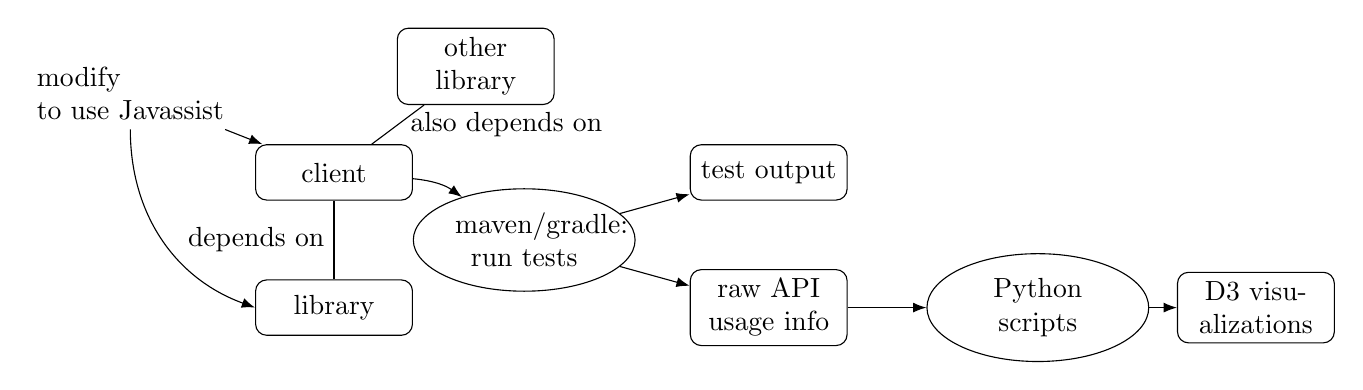
\begin{tikzpicture}
    \node[block] (client) {client};
    \node[block,below=1cm of client] (library) {library};

    \draw (library) -- node[left] (depends) {depends on} (client);

    \node[above left=.75em of client] (ja) {\begin{minipage}{7em} modify \\to use Javassist \end{minipage}};
    \draw[-Latex] (ja) -> (client);
    \draw[-Latex] (ja) to [->,bend right=35] (library.west);

    \node[block, above right=2em of client,xshift=-2em] (olib) {other library};
    \draw (client) -- node[right,xshift=.1em] (also) {also depends on} (olib);

    \node[oval,right=of depends] (test) {maven/gradle: run tests};

    \draw[-Latex] (client) to [->,bend left=15] (test);

    \node[block, right=10em of client] (output) {test output};
    \node[block, right=10em of library] (raw) {raw API usage info};

    \draw[-Latex] (test) to (output);
    \draw[-Latex] (test) to (raw);

    \node[oval, right=of raw] (Py) {Python scripts};
    \draw[-Latex] (raw) to (Py);

    \node[block, right=1em of Py] (viz) {D3 visualizations};
    \draw[-Latex] (Py) to (viz);
  \end{tikzpicture}
}
  \caption{Our instrumentation workflow. We modify existing project infrastructure to instrument clients and to run their test suites, producing raw data, which we process with our Python scripts to create D2 visualizations.}
  \label{fig:workflow}
 \end{center}
\end{figure*}


At every invoke instruction in every
loaded method which transfers control between the client and the
library, we add code to record that invoke by incrementing a counter.
We handle both static and virtual (including special, virtual,
interface, and dynamic) calls. Crossing the client/library boundary
includes callbacks from the library to the client as well as the conventional
calls from the client to the library. 

We also record field accesses (direct and reflective), dynamic proxies
and reflective calls, Java annotations, implementations,
instantiations, and casts.


\section{Visualization System}
\label{sec:vis-system}

Once we have generated data, we use a modified version
of the d3graph\footnote{\url{https://pypi.org/project/d3graph/}} library in Python to generate a d3js\footnote{\url{https://d3js.org/}}
visualization. 

VizAPI graphs are force-directed graphs based on edge weights, which we assign
according to the
frequency of interactions between the source and target nodes.
Each node is a set of one or more packages (or classes or methods) 
that belong to the same JAR. We coalesce nodes if they originate from the same 
JAR file and have the same incoming and outgoing edges. Each edge is directed 
from the source package(s) to the target package(s) and represents an interaction 
(invocations, fields, annotations, subtyping) between packages. We run a 
clustering algorithm and use its output to colour nodes based on the cluster 
that they belong to, so a colour could include nodes from the same or different JARs.
Hovering on a node shows the list of packages and 
the JAR that they belong to, 
formatted as “jar : $<$space separated list of packages$>$”.


\section{Evaluation}
\label{sec:evaluation}

We conducted a pilot study of VizAPI on an 85-project subset of the
Duets benchmarks~\cite{durieux21}. Our study included 10 libraries and
their clients. For libraries, we pick the most popular Maven repositories 
in different categories such as logging and json parsing. We pick clients partly
from popular Github repositories and partly from Duets~\cite{durieux21}.
We collect both static and dynamic data for these projects.

\begin{figure*}[h]
\begin{center}
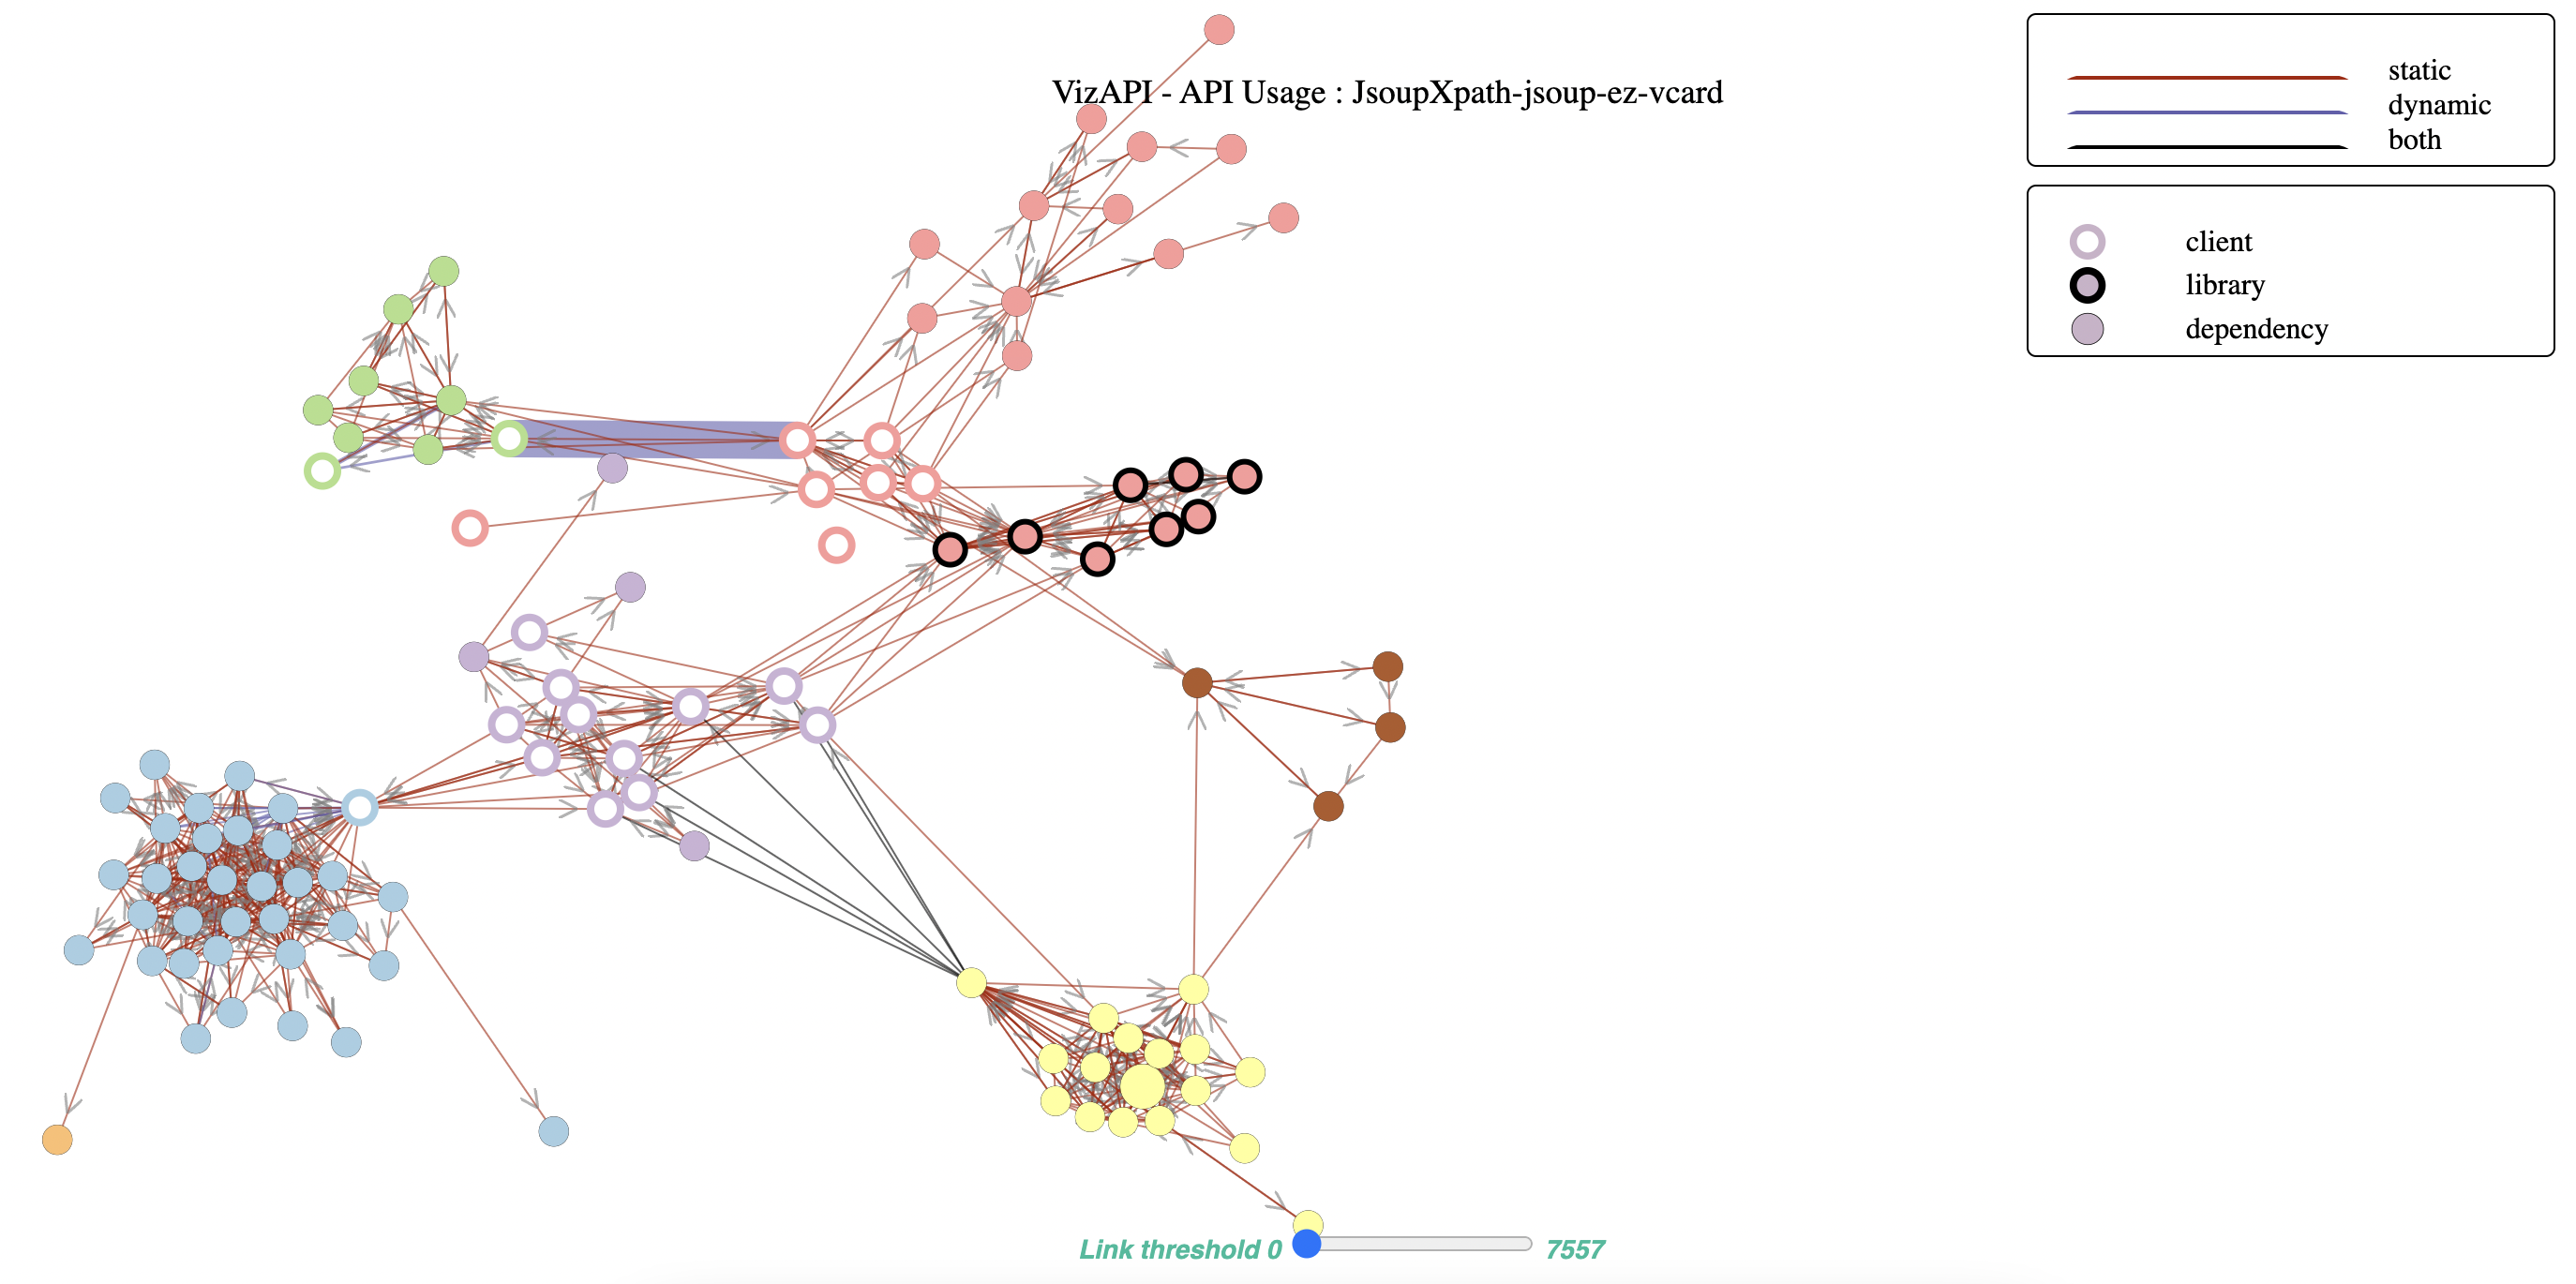
\includegraphics[scale=1,width=18cm,height=8cm]{images/usage-scenario1.png}
\caption{Usage Scenario 1: jsoup (library), JsoupXpath (client), ez-vcard (client)}
\label{fig:usagescenario1}
\end{center}
\end{figure*}

Now, we walk through an example usage scenario of VizAPI.
The graph in Figure~\ref{fig:usagescenario1} represents static and dynamic interactions of 2 clients with the jsoup\footnote{\url{https://github.com/jhy/jsoup}\label{jsoup}} library. Our clients are JsoupXpath\footnote{\url{https://github.com/zhegexiaohuozi/JsoupXpath}\label{jsoupxpath}} and ez-vcard\footnote{\url{https://github.com/mangstadt/ez-vcard}\label{ez-vcard}}.

We can start our exploration with the cluster of pink nodes. Many of these nodes belong to either JsoupXpath or jsoup. When we hover over them, the hover hints tell us that the client JsoupXpath calls directly into \texttt{org.jsoup.nodes} and \texttt{org.jsoup.select}. Notably, and as we might expect, we can see that \texttt{org.jsoup.helper} and \texttt{org.jsoup.internal} aren't called directly by JsoupXpath. This would mean that breaking changes in \texttt{org.jsoup.helper} or \texttt{org.jsoup.internal} wouldn't directly affect JsoupXpath\footnote{As a specific example, the retraction of an internal jsoup API would not break this client. Behavioural changes that are directly passed through to the external API, e.g. through delegation, can still break clients, but we can consider those to be changes in the external API.} Similarly, ez-vcard directly calls into \texttt{org.jsoup}.

ez-vcard also calls into jackson-core\footnote{\url{https://github.com/FasterXML/jackson-core}\label{jackson-core}} and jackson-databind\footnote{\url{https://github.com/FasterXML/jackson-databind}\label{jackson-databind}}, which are very tightly coupled amongst their own packages and with each other. This could mean that breaking changes in these libraries can propagate to many of their own packages.
.



\section{Discussion}
\label{sec:discussion}
Our goal when developing VizAPI was to enable 1) library developers to make better
decisions about pruning or modifying unused APIs and to refactor their
libraries; and 2) client developers to make better decisions about library
upgrades and breaking changes.

% can we talk about the use of tests a bit more? how do we miss stuff?

Note that client tests may
not adequately represent actual client behaviours; however, our use of both static
and dynamic information addresses this issue. Specifically, because we use
class hierarchy analysis for our static analysis, our visualization will present
all possible static calls---possibly too many. 
That is, the main hazard with static analysis is that our visualization may include more
static edges than are actually possible. Some of those edges could be ruled out by a more
precise call graph. Reflection aside, no static edges
are missing (our approach is ``soundy~\cite{livshits15:_in_defen_sound}'' with respect to static information). On the other hand, dynamic edges have actually been observed
on some execution; better tests could yield more dynamic edges. But even if
a dynamic edge is missing, there will be a static edge if the behaviour is possible.

Nevertheless, this preliminary work has presented two usage scenarios which we
believe promise to be useful for both client and library
developers. Consistent with the Call for Papers for the NIER track, we
have not yet carried out a formal evaluation of our VizAPI tool. We
intend to carry out further evaluation of our tool following the
techniques described by Merino et
al~\cite{merino18:_system_liter_review_softw_visual_evaluat}; in
particular, we aspire to perform experiments to establish the
effectiveness of VizAPI, where we ask users to perform software
understanding and maintenance tasks that would benefit from our tool.

%Cite a systematic literature review of software visualization evaluation (Merino et al)? Merino is PC chair and talk about how we don't have an evaluation yet but it's not required for NIER.




\end{document}
